\section{Método de pesquisa e produção assistida}
\label{sec:metodo}

\subsection{Estratégia e delimitação}

O estudo adota Design Science Research (DSR) para relacionar o problema organizacional à construção e à avaliação de um artefato \citep{hevner2004design}. As atividades da DSRM organizam identificação do problema, objetivos, desenho, demonstração, avaliação e comunicação \citep{peffers2007dsrm}. Nesta etapa, o trabalho concentra-se na pesquisa de desenho e na produção documental; a avaliação por cenários permanece prospectiva. A organização segundo DSRM não implica que todas as atividades já tenham sido concluídas.

A pesquisa possui dois objetos articulados: a especificação do GEAR e o procedimento de produção dessa especificação com IA e auditoria de conteúdo. O framework é descrito por conceitos, três domínios essenciais, rotinas e modelos de registro. O segundo objeto explicita como materiais de origem foram selecionados, sintetizados, adaptados e corrigidos. A unidade de inspeção documental é a afirmação ou prática e sua relação com a fonte. Na prova de conceito futura, a unidade de comparação será o caso de empresa sintética, mantido constante entre os três frameworks.

\begin{figure}[H]
  \centering
  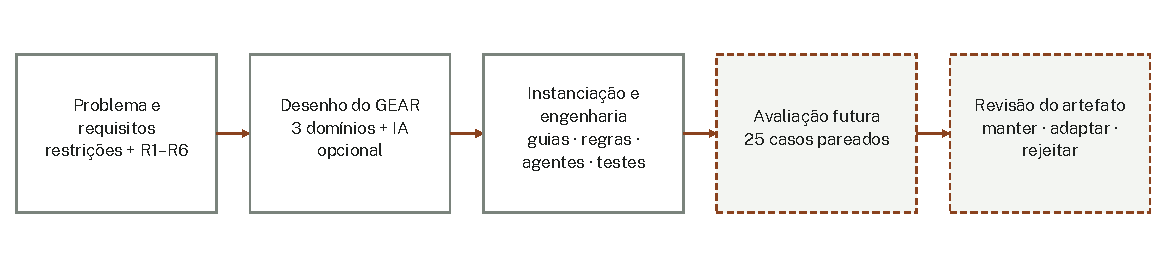
\includegraphics[width=\textwidth]{figures/generated/research-pipeline.pdf}
  \caption{Produção assistida e auditoria de conteúdo nesta etapa; prova de conceito no FrameSim e revisão por resultados em etapas futuras. A IA auxilia a produção, mas não substitui a fonte nem o julgamento autoral.}
  \label{fig:processo-pesquisa}
\end{figure}

\subsection{Leitura dirigida e requisitos de desenho}

A pesquisa partiu do projeto de TCC~I e do acervo histórico GP-PME, com leitura dirigida de estudos sobre governança em PMEs, transformação digital incremental, referências gerenciais e assistência por IA. Trata-se de uma síntese orientada ao desenho, sem protocolo de revisão sistemática exaustiva ou contagem completa de buscas, exclusões e duplicatas. Os estudos e documentos utilizados estão identificados na bibliografia e nas fichas de fontes do núcleo documental. Quando somente uma página institucional, resumo ou apresentação pública pôde ser consultado, o limite de acesso foi registrado; não se pressupõe leitura integral de livros ou normas fechadas.

O desenho adotou seis requisitos: \textbf{R1}, operação por equipe mínima e acumulação explícita de papéis; \textbf{R2}, início incremental; \textbf{R3}, cobertura conjunta de direção, execução e risco; \textbf{R4}, evidência simples por prática; \textbf{R5}, funcionamento integral sem IA; e \textbf{R6}, rastreabilidade e revisão humana quando houver IA. São critérios autorais de desenho, informados pela literatura e pelo contexto-alvo. A sua adequação dependerá da avaliação futura.

\subsection{Uso ativo de IA e auditoria de conteúdo}
\label{sec:auditoria-ia}

A IA participou da produção como instrumento de leitura, síntese e revisão. Foi usada para localizar e organizar trechos do acervo, propor minutas, comparar versões, apontar conflitos terminológicos e apoiar a preparação editorial. A auditoria de conteúdo constitui uma etapa distinta: uma sugestão plausível precisa de fonte ou de identificação explícita como adaptação autoral antes de integrar o material publicado. A assistência também pode propor verificações, mas concordância entre saídas de IA não constitui confirmação independente.

O procedimento de revisão é organizado em seis operações. (1) Identificar a fonte, versão, endereço e limite de acesso. (2) Extrair o conceito e o contexto em que a fonte o sustenta, preservando população, tarefa e período de resultados numéricos. (3) Produzir uma síntese assistida, separando citação, paráfrase e proposta local. (4) Confrontar afirmações com os trechos consultados e conferir unidades, fórmulas e consistência entre documentos. (5) Corrigir, restringir ou excluir conteúdo sem suporte e submeter escolhas à revisão autoral. (6) Registrar a versão, o destino editorial e os limites remanescentes. Essa sequência explicita o procedimento aplicado à revisão atual; não reconstrói um histórico completo de todas as interações anteriores.

A auditoria teve efeitos concretos no conteúdo. Resultados de produtividade obtidos em outras tarefas foram mantidos com seus limites, sem convertê-los em ganho esperado do GEAR. O material financeiro passou a distinguir ROI líquido, razão bruta e capacidade potencial liberada. O questionário de maturidade foi revisto para permitir atingir o nível máximo sem adoção de IA. A nomenclatura passou a fixar três domínios essenciais e assistência opcional. As fichas de origem e o \href{https://github.com/andrecodexvictor/GP-Pme/tree/codex/gear-editorial/framework/publicacao}{registro editorial} permitem examinar essas decisões e localizar suas fontes.

Os registros disponíveis são evidências de processo e de revisão, sem mensuração causal do benefício da IA. Não houve grupo de controle para a produção do material, medição uniforme do tempo de escrita ou avaliação independente de toda afirmação. Parte do histórico não registra de forma uniforme modelo, parâmetros, prompts e intervenções humanas. Esses limites impedem estimar taxa de acerto, redução de esforço ou superioridade da produção assistida. A auditoria reduz incertezas específicas; não garante ausência de erros.

\subsection{Conversão da pesquisa em práticas}

A síntese foi convertida em rotinas com evento de início, responsável, entrada, saída e evidência de encerramento. Cada prática preserva sua finalidade e declara o que foi adaptado ao contexto de equipes pequenas. Os mecanismos são conectados pelo percurso diagnosticar, decidir, executar, verificar e revisar, descrito na \cref{sec:artefato}. Guias, exemplos e modelos permitem inspecionar como a proposta poderia ser aplicada, sem serem resultados de aplicação em empresas.

A demonstração atual é documental: arquitetura, requisitos, guias e instrumentos estão disponíveis para leitura e crítica. Exemplos didáticos expõem premissas e possíveis decisões. A coerência documental e a conferência de cálculos verificam aspectos do artefato, mas não demonstram aprendizagem, adesão ou melhoria organizacional. MCPs, skills e demais integrações do repositório são mencionados como recursos associados e permanecem fora da análise e da validação deste artigo.

\subsection{Mapa de afirmações e evidências}

A \cref{tab:claim-evidence} delimita o que pode ser afirmado nesta etapa. A distinção entre registro de produção, hipótese de desenho e efeito observado orienta a escrita do manuscrito e o protocolo futuro.

\begin{table}[htbp]
  \centering
  \caption{Afirmações centrais, suporte disponível e limites.}
  \label{tab:claim-evidence}
  \small
  \begin{tabularx}{\textwidth}{@{}L{3.0cm}R R@{}}
    \toprule
    Afirmação & Suporte disponível & Limite ou evidência futura \\
    \midrule
    A governança precisa de ajuste ao contexto de PMEs & Estudos e revisão de literatura & Transferência ao recorte brasileiro exige estudo próprio \\
    O GEAR possui uma especificação documental & Núcleo, guias, modelos e fontes versionados & Usabilidade e cobertura precisam de avaliação independente \\
    A produção usou IA e auditoria de conteúdo & Declaração de uso, fontes e registros de revisão & Histórico incompleto; sem medida causal de benefício da IA \\
    O GEAR pode reduzir esforço de coordenação & Hipótese derivada de rotinas e artefatos compactos & Prova de conceito com alternativas comparáveis \\
    O GEAR melhora resultados organizacionais & Não afirmado nesta versão & Evidência de campo além da simulação \\
    \bottomrule
  \end{tabularx}
\end{table}
